\documentclass[10pt,a4paper]{report}
\usepackage[a4paper, total={6in, 8in}]{geometry}
\usepackage[utf8]{inputenc}
\usepackage{amsmath}
\usepackage{amsfonts}
\usepackage{amssymb}
\usepackage{graphicx}

\begin{document}

{\LARGE \center Advanced Computer Graphics \\ Homework 6\\ Particle System Part 2\\}
{\large \center Group 8\\ Damien Doy - 244206\\
Jason Racine - 244270\\
Alexandre Veuthey - 224295\\
}

\section*{Computation of the triangle area forces}
In order to find the force at each vertice of the triangle we have to find the following partial derivative (as stated in the lecture):\\
$F_i=-\frac{\partial EA(x_0,x_1,x_2)}{\partial x_si}$ 
where 
$EA(x_0,x_1,x_2)=0.5k_A(area(x_0,x_1,x_2)-A)^2$\\
and \\
$area(x_0,x_1,x_2)=0.5((x_1.x-x_0.x)(x_2.y-x_0.y)-(x_2.x-x_0.x)(x_1.y-x_0.y))$\\
By solving these equations, we get:\\\\
$Fi=-\frac{\partial EA(x_0,x_1,x_2)}{\partial x_i}=k_A(area(x_0,x_1,x_2)-A)
\frac {\partial area(x0,x1,x2)}{\partial x_i}$\\\\
And by solving the partial derivative we get the following forces for each particles:\\\\
$F_0=-0.5dEA(x_1.y-x_2.y, x_2.x-x_1.x)\\
F_1=-0.5dEA(x_2.y-x_0.y, x_0.x-x_2.x)\\
F_2=-0.5dEA(x_0.y-x_1.y, x_1.x-x_0.x)\\
$where $dEA=k_A(area(x_0,x_1,x_2)-A)$

\section*{Computation of the Jacobian}

\subsection*{Gravity}
Let's begin with the gravitation force, which is defined as\\
$
F_G=\begin{pmatrix}
0 \\
-Gm \\
\end{pmatrix}
$\\
Since the force of gravity does not depend on the position of the particle, the 2x2 Jacobian
of this force by the particle position is a null matrix and doesn't have to be added to the solver\\
\subsection*{Centre force}
The center force is defined as:\\
$
F_C=\begin{pmatrix}
-Cx\\
-Cy\\
\end{pmatrix}
$\\
And thus, the jacobian of this force is:\\
$
J_C=\begin{pmatrix}
-C && 0\\
0 && -C\\
\end{pmatrix}
$\\
\subsection*{Force-based collisions}
The force based collision is applied to the particle only when\\
$xn_x+yn_y+n_z-p_{radius} < 0$ where $x$ and $y$ are the position of the particle, and $n_x$, $n_y$ and $n_z$ are the parameters of the line equation. Then the force is:\\
$
F_{Col}=\begin{pmatrix}
-n_x(xn_x+yn_y+n_z-p_{radius})k_{col}\\
-n_y(xn_x+yn_y+n_z-p_{radius})k_{col}
\end{pmatrix}
=
\begin{pmatrix}
-k_{col}(xn_x^2+yn_xn_y+n_xn_z-p_{radius}n_x)\\
-k_{col}(xn_xn_y+yn_y^2+n_yn_z-p_{radius}n_y)
\end{pmatrix}
$\\\\
Then the jacobian is\\\\
$
J_{Col}=\begin{pmatrix}
-k_{col}n_x^2 	&& -k_{col}n_xn_y\\
-k_{col}n_xn_y 	&& -k_{col}n_y^2
\end{pmatrix}
$
\subsection*{Damped-spring forces}
TODO\\
\subsection*{Area preservation forces}
TODO\\

\section*{Computation of the equilibrium force}
In order to distribute the particles on the screen, we added a force that acts on every particles. They repulses themselves like same polarity charges in electromagnetism.\\
To avoid a unstable system and to reduce the computation time, we limited this force to a certain radius around each particle. This radius is equals to\\
$radius = C(\frac{1}{dist}-1)*normal_{p_0,p_1}$ where $dist \in {0, 1}$ is the distance between two particles normalized. $C$ is a constant that makes the equilibrium force stronger or weaker.\\
Here is a graph of this function:\\
\begin{center}
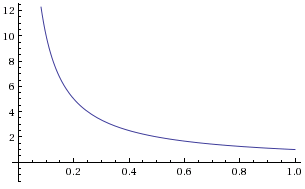
\includegraphics[scale=0.5]{graph_equib.png}\\
\end{center}
The advantage of a strong force, is that particles will distribute uniformly faster, but a great force will make the system go unstable.\\
A weak force can also be advantageous, particles will move slower to their positions but there is less risk of particles flying off.\\
Here we tested the equilibrium force on 30, 100, 250 particles, with verlet integration and impulse based forces:\\
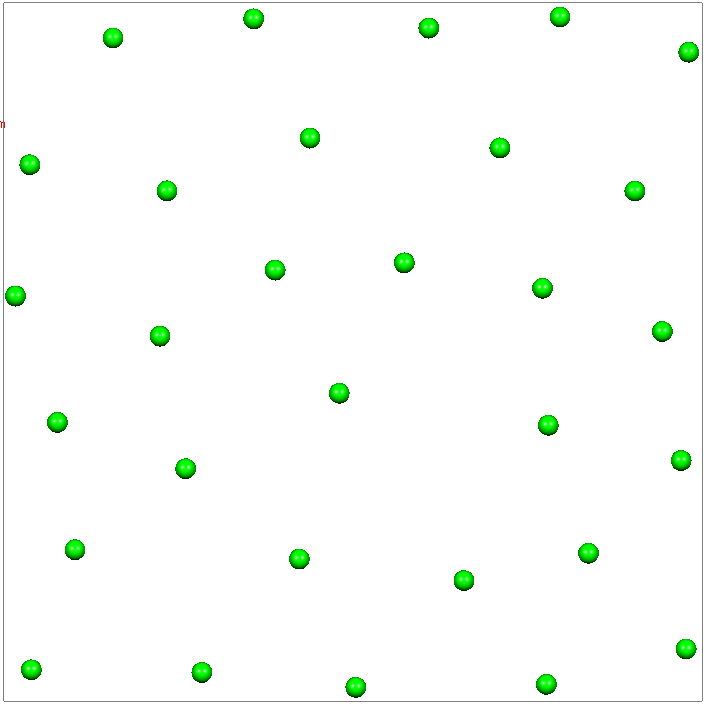
\includegraphics[scale=0.25]{30.png}
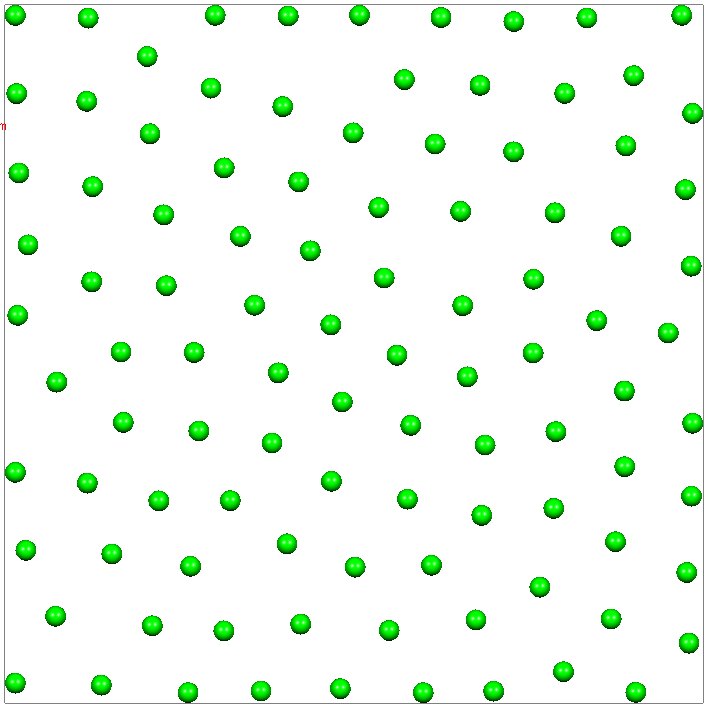
\includegraphics[scale=0.25]{100.png}\\
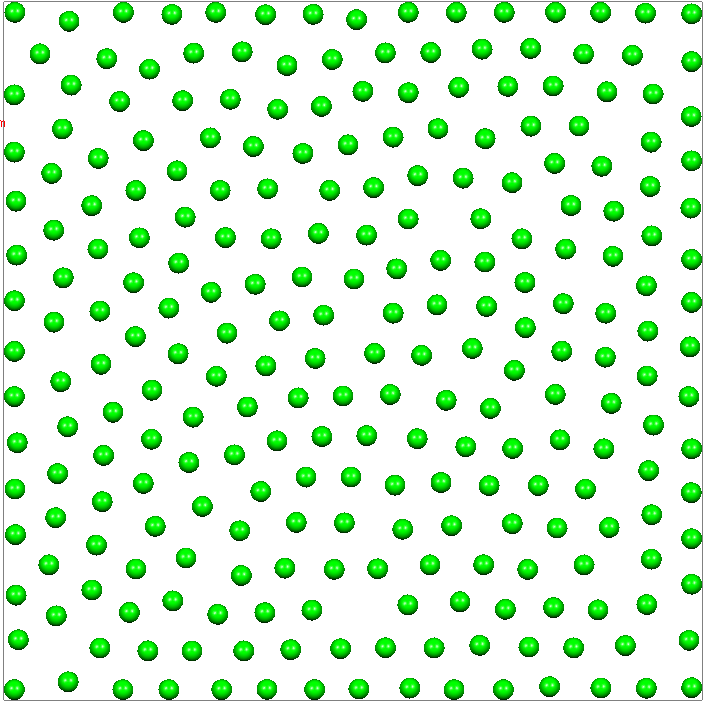
\includegraphics[scale=0.25]{250.png}

\end{document}